\documentclass{beamer}

\usepackage[francais]{babel}
\usepackage[utf8]{inputenc}
\usepackage{amsmath}
\usepackage{amssymb}
\usepackage[T1]{fontenc}
\usepackage{bm}
\usepackage[french]{algorithm2e}
\usepackage{graphicx}
\usepackage{natbib}
\setbeamertemplate{footline}[frame number]
\beamertemplatenavigationsymbolsempty



\title{Équité dans le Filtrage Collaboratif}
\author{Hector Dang-Nhu \& Cyrine Hlioui \& Romain Warlop}
\renewcommand{\phi}[0]{\varphi}
\newcommand{\norm}[1]{\left\lVert#1\right\rVert}

\begin{document}
\begin{frame}
  \maketitle
\end{frame}
\section{Introduction}
\begin{frame}{Introduction}
  \begin{itemize}
    \item Système de Recommandation : estimer la manièr dont un utilisateur $i$ peut réagir à un produit $j$
    \item Filtrage Collaboratif : utiliser les réactions des utilisateurs pour faire des recommandations
  \end{itemize}
\end{frame}
\begin{frame}{Factorisation de Matrice}
  $$\min_{U,M}\sum_{i,j} (r_{i,j} - U_iM_j^T)^2 + \mu\left(\sum_i||U_i||^2+ \sum_j||M_j||^2\right)$$
  $U$ la matrice des utilisateurs, $M$ la matrice des produits
\end{frame}

\begin{frame}{Mesures d'équités}
  Parité démographique, avec $A$ l'attribut protégé et $\hat Y$ la décision binaire :
  $$P(\hat Y = 1 | A = 0) = P(\hat Y = 1 | A = 1) $$
  Opportunités égales avec $A$ l'attribut protégé, $\hat Y$ la décision binaire et $Y$ l'étiquette réelle :
  $$\forall y, P(\hat Y = 1 | A = 0, Y = y) = P(\hat Y = 1 | A = 1, Y = y) $$
  Importance pour des questions de lutte anti-discrimination, entre autres.
\end{frame}
\begin{frame}{Mesures d'équités côté fournisseur de contenu}
  Problème : équité pour les artistes ou les produits
\end{frame}

\section{Définition du problème}
\begin{frame}{Métriques en Top-K}
$$\phi(S) = \sum_i\sum_{j\in S_i}r_{i,j}$$
$$\mathcal{E}(S) = \sum_{c=1}^C\left(\frac{1}{nK}\sum_i\sum_{j\in S_i}\left[\bm{1}_{j\in P_c}\right] - p_c\right)^2$$
$r_{i,j}$ le score donné par l'utilisateur $i$ au produit $j$\\
$P_c$ l'ensemble des produits de la catégorie $c$\\
$p_c$ la proportion cible pour cette catégorie\\
$S_i$ est l'ensemble de taille $K$ de recommandations pour l'utilisateur $i$
\end{frame}
\begin{frame}{Métriques en Top-1}
$$\phi(S) = \sum_ir_{i,S(i)}$$
  $$\mathcal{E}(S) = \sum_{c=1}^C\left(\frac{1}{n}\sum_i\left[\bm{1}_{S(i)\in P_c}\right] - p_c\right)^2$$
  $S$ est désormais une fonction qui à un utilisateur $i$ sa recommandation $S(i)$.
\end{frame}
\section{Algorithmes proposés}
\begin{frame}{Recommandation probabiliste pour chaque utilisateur}
  $$\Pr(S(i) \in P_c)\propto \begin{cases} p_c & \text{ s'il peut y avoir une recommandation dans }P_c  \\ 0 & \text{autrement.} \end{cases}$$
  Pour chaque $i$, on prend la meilleure estimation de $P_c$\\
  ~\\
  En $O(nm)$ mais peut être ramené à un pré-calcul en $O(nm\log(nm))$ et une exécution en $O(n\log(m))$.
\end{frame}
\begin{frame}{Recommandation par proportions globales}
\begin{algorithm}[H]
   \While{ il y a des recommandations à faire}
   {
    On prend la catégorie avec la plus grande différence en défaut d'éléments dans les recommandations actuelles\;
    On prend la paire $(i,j)$ de la catégorie avec le plus grand $\hat r$\;
    La paire $(i,j)$ devient la recommandation\;
   }
  \end{algorithm}
  ~\\
  En $O(nm\log(nm))$ avec des tas
\end{frame}
\begin{frame}{Optimisation par pénalisation par l'équité}
\begin{align*}
  \min_{U,M}\sum_{i,j} (r_{i,j} - U_iM_j^T)^2 & + \mu\left(\sum_i||U_i||^2+ \sum_j||M_j||^2\right)\\
  & + \lambda \norm{ T - \frac{1}{n}\bm{1}_{n}UM^TC}^2
\end{align*}
$U$ la matrice des utilisateurs, $M$ la matrice des produits\\
$T$ le vecteur des proportions cible des produits\\
$C$ la matrice telle que $C_{j,c}=\bm 1_{j\in P_c}$\\
$\lambda$ et $\mu$ deux hyper paramètres\\
\end{frame}
\section{Résultats}
\subsection{Remarques sur l'implémentation}
\begin{frame}{Implémentation}
  \begin{itemize}
    \item On utilise le package \verb?surprise? pour les systèmes de recommandations
    \item On utilise le modulo de l'id des produits pour savoir leur catégorie
    \item $p_c\propto 2(c+1)$
    \item On utilise SVD pour estimer les $r_{ij}$
  \end{itemize}
\end{frame}
\subsection{Similarité}
\begin{frame}{Similarité Totale}
  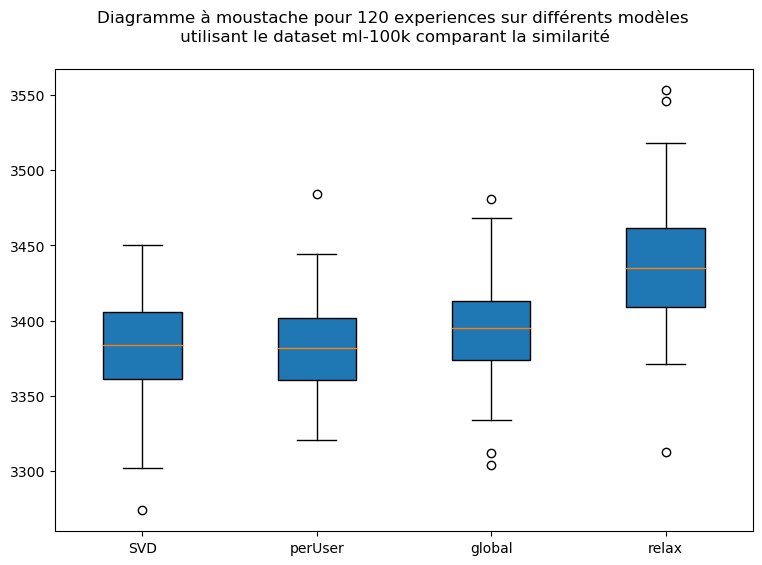
\includegraphics[width = 10cm]{sim1}

\end{frame}
\subsection{Équité}
\begin{frame}{Terme d'Équité}
  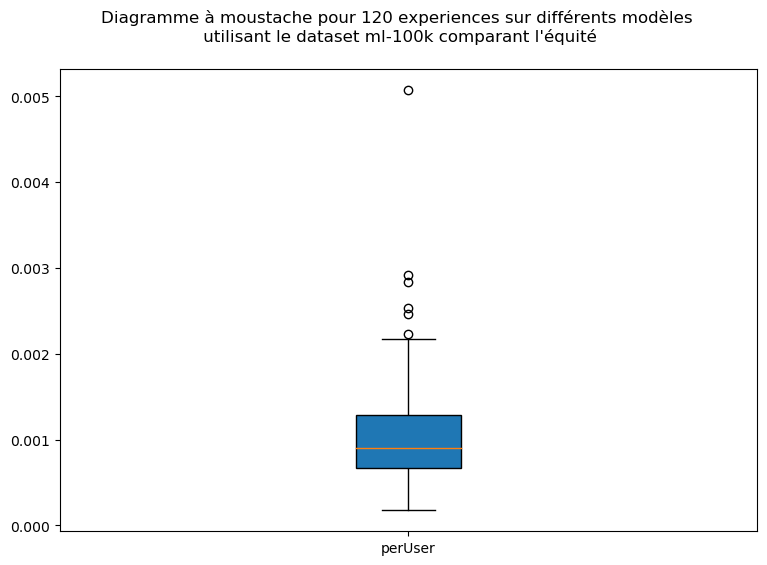
\includegraphics[width = 5cm]{eq2}
  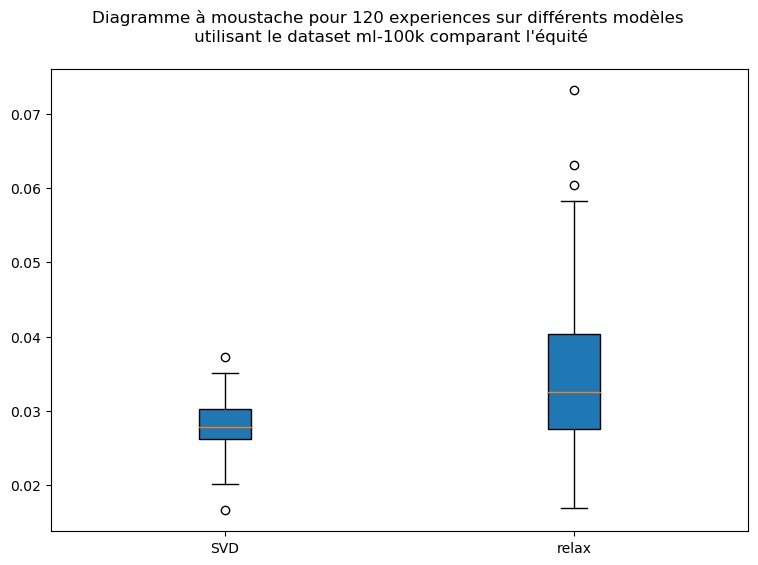
\includegraphics[width = 5cm]{eq3}
\end{frame}
\subsection{Temps d'exécution}
\begin{frame}{Temps d'exécution}
  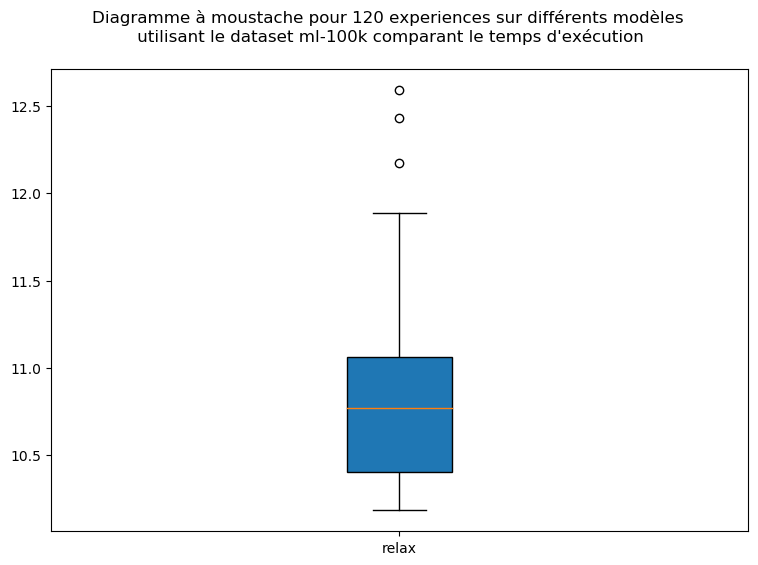
\includegraphics[width = 5cm]{t1}
  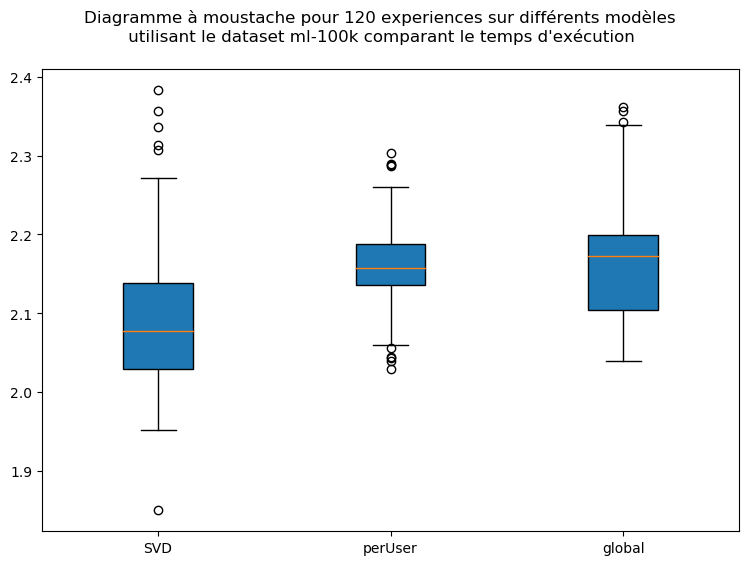
\includegraphics[width = 5cm]{t2}
\end{frame}
\section{Pistes d'amélioration}
\begin{frame}{Pistes d'amélioration}
  \begin{itemize}
    \item Pondération des probabilités par la similarité pour la recommandation par utilisateur
    \item Amélioration de la descente de gradient et utilisation de softmax ou de normalisation dans le terme de la perte d'équité
    \item Relaxation convexe
    \item Heuristiques pour un algo qui optimise brutalement avec une contrainte d'équité
    \item Top-K
  \end{itemize}
\end{frame}
\nocite{toward,netflixmoney,yao2017parity,pleiss2017fairness}
\begin{frame}{Bibliographie}
  \bibliographystyle{plain}
  \bibliography{projet}
  %\url{https://github.com/boolon/Projet-Equite}
\end{frame}
\begin{frame}
  Merci de votre attention
\end{frame}

\end{document}
